\documentclass[]{article}

%opening
\title{4M24 CW - High-Dimensional MCMC}
\author{Candidate: 5562E}

%packages
\usepackage[margin=0.5in]{geometry}
\usepackage[export]{adjustbox}
\usepackage{mathtools}
\usepackage{graphicx}
\usepackage{amsmath}
\usepackage{amssymb}
\usepackage{hyperref}
\usepackage{caption}
\usepackage{subcaption}
\usepackage{parskip}
\usepackage{listings}
\usepackage{pdfpages}
\usepackage{bbm}

%package setup
\graphicspath{{./img/}}
\DeclareMathOperator*{\argmax}{arg\,max}
\DeclareMathOperator*{\argmin}{arg\,min}

%custom commands
\newcommand{\figwidth}{0.6\linewidth}
\newcommand{\Fcal}{\mathcal{F}}
\newcommand{\idft}{\mathcal{F}^{-1}}
\newcommand{\Xcal}{\mathcal{X}}
\newcommand{\Ncal}{\mathcal{N}}
\newcommand{\Acal}{\mathcal{A}}
\newcommand{\Bcal}{\mathcal{B}}
\newcommand{\cmplx}{\mathbb{C}}
\newcommand{\Lcal}{\mathcal{L}}
\newcommand{\Mcal}{\mathcal{M}}
\newcommand{\indep}{\perp \!\!\! \perp}
\newcommand{\iid}{\stackrel{iid}{\sim}}
\newcommand{\betaml}{\hat{\beta}^{ML}}
\newcommand{\Expect}{\mathbb{E}}
\newcommand{\xbold}{\boldsymbol{x}}
\newcommand{\ubold}{\boldsymbol{u}}
\newcommand{\vbold}{\boldsymbol{v}}
\newcommand{\epsbold}{\boldsymbol{\epsilon}}


%section numbering
\renewcommand{\thesubsection}{\alph{subsection}}

\begin{document}


\includepdf[pages={1}]{4M24-Coversheet.pdf}

\setcounter{page}{1}
\maketitle

\begin{abstract}
	This report outlines the result of the 4M24 coursework on high-dimensional Markov Chain Monte Carlo (MCMC).
\end{abstract}

\tableofcontents

\section{Introduction}

\section{Simulation}
\subsection{Sampling from a Gaussian Process}

We begin with a Gaussian Process (GP) defined on a 2D domain $\xbold \in [0, 1]^2$. The realisations from this process are denoted $\ubold \sim \Ncal(0, C)$ where $C_{ij} = k(\xbold_i, \xbold_j)$ and k is the Squared Exponential (SE) covariance function with length parameter $l$:
%
\begin{equation}
	k(\xbold, \xbold ') = \exp \left( \frac{-||\xbold - \xbold '||^2}{2l^2}\right)
	\label{eqn:k-defn}
\end{equation}

If we specify the latent variables $\{\xbold_i\}_{i=1}^N$, then we can compute $C$ and hence fully specify the prior on $u$. We choose to place $\{x_i\}_{i=1}^N$ on a $D \times D$ grid with equal spacing, starting at $(0,0)$ and ending at $(1,1)$. Obviously, we require $N = D^2$.

We can now plot the $u$-surface atop this grid by ensuring that for each $i \in \{1 \dots N\}$, $u_i$ denotes the Z-position and $\xbold_i$ the X-Y-position. We can then investigate the effect of varying the length-scale parameter $l$. Three settings of $l$ and the associated plots are given in figure \ref{fig:l-effect} for $D=16$.
%
\begin{figure}[!h]
	\centering
	\begin{subfigure}{0.32\linewidth}
		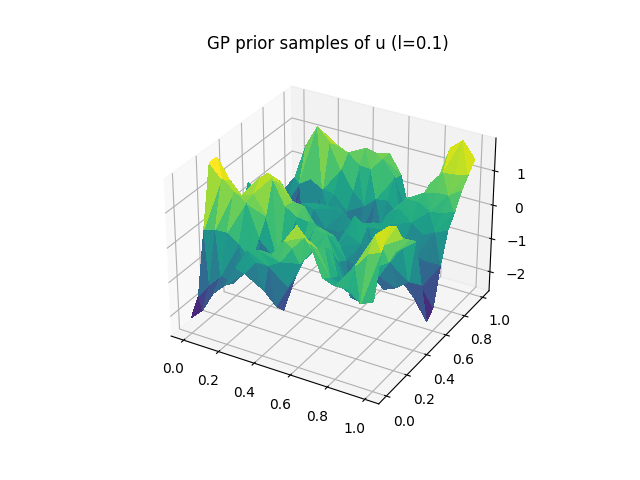
\includegraphics[width=\linewidth]{u-small.png}
		\caption{Small $l=0.1$}
	\end{subfigure}
	\begin{subfigure}{0.32\linewidth}
		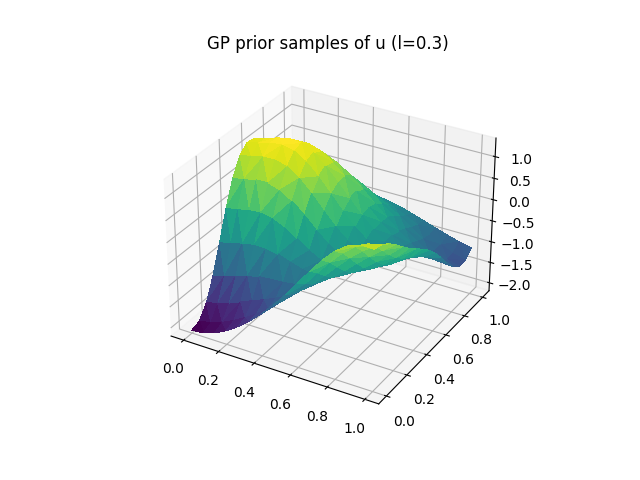
\includegraphics[width=\linewidth]{u-med.png}
		\caption{Medium $l=0.3$}
	\end{subfigure}
	\begin{subfigure}{0.32\linewidth}
		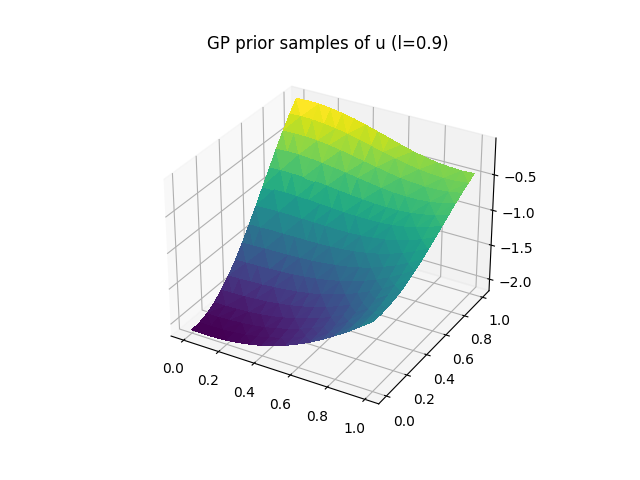
\includegraphics[width=\linewidth]{u-big.png}
		\caption{Large $l=0.9$}
	\end{subfigure}
	\caption{Samples from GP prior for varying length scales ($D=16$)}
	\label{fig:l-effect}
\end{figure}

We now proceed to make $M$ random draws (denoted by the $M \times 1$ vector $\vbold$) from these samples $\ubold$ with additive Gaussian noise $\epsbold \sim \Ncal(0, I)$. The subsampling factor $f$ is defined as $f \coloneqq N / M$. The draws can be computed as follows:
%
\begin{equation}
	\vbold = G \ubold + \epsbold
	\label{eqn:v-defn}
\end{equation}

Where $G$ is an $M \times N$ matrix with a single one in each row in a random location (without repetition) and rest zeros. The result is that the observations $\vbold$ are a jumbled subsample of $\ubold$ with additive noise $\epsbold$. We can plot the data overlaid on the original prior samples by simply matching each entry of $\vbold$ back to the coordinate it was selected from. The result is plotted on figure \ref{fig:v-on-u}.
%
\begin{figure}[!h]
	\centering
	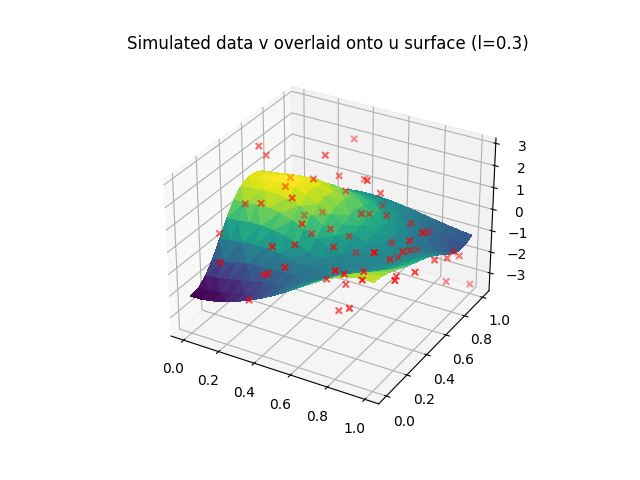
\includegraphics[width=\figwidth]{v-overlay.png}
	\caption{$\vbold$ (red crosses) overlaid on $\ubold$-surface ($f=4, D=16, l=0.3$)}
	\label{fig:v-on-u}
\end{figure}

We observe $M=N/f=16^2/4=64$ samples contained in the $\vbold$ vector. These are equally likely to appear above or below the $\ubold$-surface as the noise has zero mean. The noise variance for each data-point is of similar magnitude to the variation in the surface ($\sigma^2 = 1$) so some crosses appear relatively far away from the surface. Moreover, as the subsampling is random, the $\vbold$-points appear at randomly chosen (but distinct) locations X-Y plane.

\subsection{Log probabilities and MCMC}

The log prior can be calculated simply, through manipulation of the Gaussian pdf:
%
\begin{align}
	\ln p (\ubold) &= \ln \Ncal(\ubold; 0, C) \nonumber \\
	&= \ln \frac{1}{(2\pi)^{N/2} |C|^{1/2}} \exp \left( - \frac{1}{2} \ubold^T C^{-1} \ubold \right) \nonumber \\
	&= - \left( \frac{N}{2} \ln 2\pi + \frac{1}{2} \ln |C| + \frac{1}{2} \ubold^T C^{-1} \ubold \right)
	\label{eqn:log-prior}
\end{align}

Likewise, $\vbold | \ubold$ is also a Gaussian such that $\vbold |\ubold \sim \Ncal(G\ubold, I)$ (see equation \ref{eqn:v-defn}). By comparison with the form of equation \ref{eqn:log-prior}, we can jump straight to the log-likelihood, noting that $\ln |I| = 0$:
%
\begin{equation}
	\ln p(\vbold | \ubold) = - \left( \frac{M}{2} \ln 2 \pi + \frac{1}{2} \left(\vbold - G\ubold \right)^T \left(\vbold - G\ubold\right)\right)
\end{equation}

\textbf{Words}: XX

\end{document}
